\documentclass{article}
\usepackage{float}
\usepackage{pdfpages}
\usepackage{graphicx}
\graphicspath{{C:/Users/Brayden/Projects/PEPS-Data/}{.}}
%\usepackage{adjustbox}
%\usepackage[export]{adjustbox}
\usepackage{geometry}
\usepackage{pdflscape}
\usepackage{fullpage}
\usepackage{amsmath} % for some of the mathematical symbols
\usepackage{amsthm}  % for the Question environment
\usepackage{amssymb} % for the \mathbb command
\usepackage{latexsym,amscd,amsfonts}


\setlength{\textwidth}{6.5in}    % adjusted text sizes
\setlength{\oddsidemargin}{0.0in}
\setlength{\evensidemargin}{0.0in}
\setlength{\textheight}{9in}
\setlength{\topmargin}{0in}
\setlength{\headheight}{0in}
\setlength{\headsep}{0in}

\newcommand{\bra}[1]{\left \langle #1 \right |}
\newcommand{\ket}[1]{\left |#1 \right \rangle}
\newcommand{\braket}[2]{\left \langle #1 \middle |#2 \right \rangle} 
\newcommand{\braopket}[3]{\left \langle #1 \middle |#2 \middle | #3 \right \rangle} 
\newcommand{\bratext}[1]{\left \langle \text{#1} \right |}
\newcommand{\kettext}[1]{\left |\text{#1} \right \rangle}
\newcommand{\brakettext}[2]{\left \langle \text{#1} \middle |\text{#2} \right \rangle}

\newcommand{\vbra}[1]{\left ( #1 \right |}
\newcommand{\vket}[1]{\left |#1 \right )}
\newcommand{\vbraket}[2]{\left ( #1 \middle |#2 \right )} 

\title{Featureless Boson States with PEPS}
\author{Brayden Ware}
\date{August 2014}

\begin{document}

\maketitle


The proposed featureless boson insulator state has a wavefunction given by 

\begin{equation}
\ket{\psi} = \prod\limits_{R} \sum\limits_{i \in R} b^{\dagger}_{i} \ket{0}
\label{eq:def}
\end{equation}

where $R$ refers to each hexagonal plaquette of a honeycomb lattice, and $i \in R$ referes to the honeycomb sites adjacent to the plaquette $R$. It has been argued in  \cite{Kimchi2012-lr} that this state represents a featureless Mott insulating phase of bosons on the honeycomb lattice.

Three variations:
\begin{itemize}
\item \emph{Soft-core boson}

This is the usual boson operator, which acts on the on-site boson number basis

$$ b^{\dagger} \ket{N} = \sqrt{N+1} \ket{N+1} $$

with the commutation relations 

$$ [b_i, b_j^{\dagger}] = \delta_{ij}.$$

The on-site Hilbert space $ \mathbb{H} = \text{span} ( \ket{N}, N \in \mathbb{Z} )$ is infinite-dimensional; but because each vertex is attributed at most one boson from each of its adjacent hexagons, the state lives in the subspace with at most 3 bosons on each site. The on-site Hilbert space can be truncated to 4-dimensions, where the boson creation operator is represented as

$$b^{\dagger} =  \left( \begin{array}{cccc}
0 & 0 & 0 & 0 \\
1 & 0 & 0 & 0 \\
0 & \sqrt{2} & 0 & 0 \\
0 & 0 & \sqrt{3} & 0 \end{array} \right), 
$$

\item \emph{Hard-core boson}

This is the state obtained by taking the soft-core boson state and projecting on every site to the subspace of at most 1 boson on each site. Because of this projection, the on-site Hilbert space can be taken to be the 2-dimensional subspace $\mathbb{H} = \text{span}(\ket{0}, \ket{1})$, with the boson creation operator represented on this subspace as:

$$b^{\dagger} =  \left( \begin{array}{cccc}
0 & 0 \\
1 & 0 \end{array} \right) 
$$

Note that the boson operator restricted to this subspace clearly does not satisfy the usual boson commutation relations. 

\item \emph{Large-N boson and other variations}

A different wavefunction can be produced by instead starting with $N$ bosons on each site before applying the plaquette boson creation operators - instead of with $0$ bosons as above:
$$
\ket{\psi} = \prod\limits_{R} \sum\limits_{i \in R} b^{\dagger}_{i} \ket{N}.
$$

This would be a candidate wavefunction for a incompressible state with boson density $N+\frac{1}{2}$ per site. We will argue that wavefunctions with different $N$ can be smoothly connected without a phase transition, so we will not need to study the physics of each independently. 

The on-site Hilbert space is again effectively 4-dimensional:  $ \mathbb{H} = \text{span} ( \ket{N}, \ket{N+1}, \ket{N+2}, \ket{N+3} )$. On this truncated Hilbert space the boson creation operator is represented as 

$$
b^{\dagger} 
=  
\left( \begin{array}{cccc}
0 & 0 & 0 & 0 \\
\sqrt{N+1} & 0 & 0 & 0 \\
0 & \sqrt{N+2} & 0 & 0 \\
0 & 0 & \sqrt{N+3} & 0 \end{array} \right) 
$$

In the limit N becomes very large,

$$
\frac{b^{\dagger}}{\sqrt{N+1}} 
=  
\left( \begin{array}{cccc}
0 & 0 & 0 & 0 \\
1 & 0 & 0 & 0 \\
0 & \sqrt{1+\frac{1}{N+1}} & 0 & 0 \\
0 & 0 & \sqrt{1+\frac{2}{N+1}} & 0 \end{array} \right) 
\approx 
\left( \begin{array}{cccc}
0 & 0 & 0 & 0 \\
1 & 0 & 0 & 0 \\
0 & 1 & 0 & 0 \\
0 & 0 & 1 & 0 \end{array} \right) 
$$

The $\sqrt{N+1}$ factor only changes the norm of the wavefunction, which is of no concern. After rescaling, all of these wavefunctions can be generated using Equation \ref{eq:def} with the replacement
 
\begin{equation}
b^{\dagger} = 
\left( \begin{array}{cccc}
0 & 0 & 0 & 0 \\
1 & 0 & 0 & 0 \\
0 & \sqrt{2} b_1 & 0 & 0 \\
0 & 0 & \sqrt{3} b_2 & 0 \end{array} \right) 
\label{eq:b}
\end{equation}

where $b^{\dagger}$ acts on a dimension 4 Hilbert space at each site with appropriate values of $b_1$ and $b_2$.

\end{itemize}


Similarly, starting with $N$ bosons at each site, but using the boson annhilation operator $b_i$ in place of the boson creation operator $b^{\dag}_i$ in Equation \ref{eq:def} gives a different family of wavefunctions. These can be represented in the form of Equation \ref{eq:b}.


Using instead the languague of spin, we can generate candidate wavefunctions for magnetization plateaus with half-integer magnetization $m = < S_z > = m_0 + \frac{1}{2}$ per site. This is done using a Hilbert space of spin-$S$ at each site, starting each site in the state $\ket{S^z = m_0}$, and using spin raising/lowering operators $S_{\pm}$ in place of boson operators. These can be represented in the form of Equation \ref{eq:b} as well. In the limit $S \rightarrow \infty$, these states become equivalent to states generated by boson creation or annhilation operators.

The location of a of these states on the $b_1$-$b_2$ plane can be seen in Figure \ref{fig:bosons}. We find that the correlation length stays bounded everywhere in this region $0<=b_2 <= b_1$ and that it monotonically increases as you approach $b_1 = b_2 = 0$. This could justify using analytical techniques available at particular points in the plane - i.e., large-S expansion can be used at the large-N boson state (also described as $S -> \infty$ $m_0 = 0$ ). Itamar's notes derive a rotor model that describes this point.


%This operator represents $P b^{\dagger} P$ or $P S^+ P$, where $P$ is a projector to the truncated Hilbert space, not a boson operator with canonical commutation relations.  All calculations below are done on the truncated Hilbert space, so any formulas below should be assumed to have projectors $P$ at the appropriate locations. 

\begin{figure}[hbctp]
\begin{center}
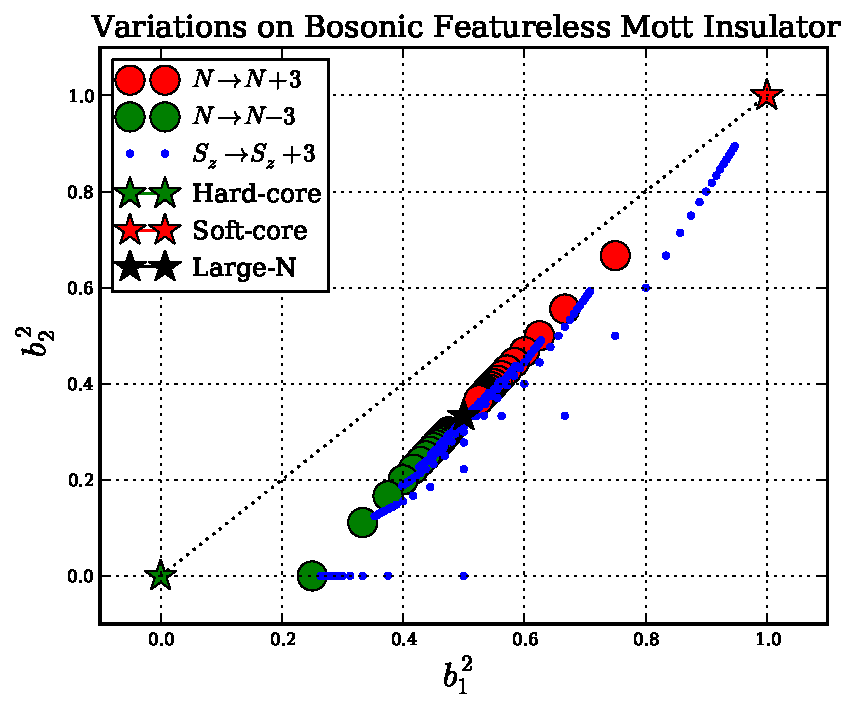
\includegraphics[width=6in]{{summary/boson_variations2.pdf}}
\end{center}
\caption{Plot of $b_1$ and $b_2$ for physically inspired variations on the featureless bosonic state. States colored red(green) - start with a vacuum of n bosons at each site and apply creation(destruction) operators. States colored blue have a spin-s Hilbert space on each site, start with all sites in the $\ket{S_z = m}$ state, and use spin-raising operators instead of boson-creation operators. }
	\label{fig:bosons}
\end{figure}

We will construct these wavefunctions as projected entangled pair states (PEPS) and the parameters $b_1$ and $b_2$ will appear in the site PEPS tensor. We then use these PEPS wavefunctions to numerically compute  correlation functions and entanglement properties, focusing in-particular on the cases of the soft-core and hard-core bosons. After discussing these correlation functions in more detail, we argue that these states are in the same phase by looking at the correlation length as $b_1$ and $b_2$ continuously vary between the hard-core and soft-core boson states.

\section{Methods}

\subsection{Making the PEPS}
Each plaquette creation operator $\sum\limits_{i \in R} b^{\dagger}_{i}$ can be written as a matrix product operator (MPO) acting on the six sites of a single hexagonal plaquette. By applying these MPOs for all plaquettes to the initial product state wavefunction $\ket{\mathbf{0}}$, we can construct a representation of the wavefunction as a PEPS with bond dimension 4 on the honeycomb lattice. 

If we define the tensor
$$
B^i_{\alpha \beta} = \left\{
     \begin{array}{lr}
       \delta_{\alpha \beta} & : i = 0\\
       (b^{\dagger})_{\alpha \beta} & : i = 1
     \end{array}
   \right\}
$$
in which the application of the creation operator is controlled by the state of the virtual qubit $i$,
then the matrix elements of the plaquette boson creation operator can be specified by a trace over one virtual qubit per site $x$ adjacent to the plaquette:

\begin{equation}
\braopket{\{\alpha_x\}}{\sum\limits_{x \in R} b^{\dagger}_{x}}{\{\beta_x\}} =
 \sum\limits_{\{i_x\}} W^{i_0 i_1 i_2 ...} \prod\limits_x B^{i_x}_{\alpha_x \beta_x} 
\label{eq:plaquette}
\end{equation}

The tensor $W^{i_0 i_1 i_2 i_3 i_4 i_5}$ which represents the state of the virtual qubits should be taken as the W-state, 
$$ W^{\{i_x\}}  = \left\{ \begin{array}{lr}
													1  : & \sum\limits_x i_x = 1 \\
													0  : & \text{else}
													\end{array}
											\right\},
$$
so that the trace results in 6 terms, each which acts as a creation operator on one site and identity on the other five sites.

The whole state can thus be represented as a contraction over all internal labels of a product of a $W$-tensor for every plaquette and a rank-4 site tensor $D$ for each site, where
$$
D_{p}^{i_0 i_1 i_2} = \sum\limits_{\alpha \beta} B^{i_0}_{p \alpha}B^{i_1}_{\alpha \beta} B^{i_2}_{\beta 0}.
$$
The internal labels $i_0$, $i_1$, $i_2$ connect the site to the adjacent plaquettes, and the label $p$ represents the physical site Hilbert space. The coefficients are
\begin{equation}
\braket{\{p_x\}}{\psi} = \sum\limits_{\{i\}} \prod\limits_{R} W^{\{i\}_R} \prod\limits_x D_{p_x}^{\{i\}_x}.
\label{eq:PEPS}
\end{equation}

This tensor network contraction scheme is different than PEPS because the $W$ tensors exist not on the sites but the plaquettes - and sites are connected to adjacent plaquettes, not to adjacent sites. To rewrite the state in a PEPS representation, one should express the W-state as a matrix product state - i.e. as a tensor contraction of 6 tensors, each of which involving only one of the 6 virtual qubits $i_j$. These new tensors can be contracted into the on-site tensors, leaving only tensors on the sites. The bond dimension of the resulting PEPS representation is the square of the bond dimension of the MPS representation of the W-state. 

A bond-dimension 2 representation of the W-state is given by
$$
W^{i_0 i_1 i_2 i_3 i_4 i_5} = \sum\limits_{abcde} W^{i_0 a}_{1} W^{i_1 b}_{a} W^{i_2 c}_{b} W^{i_3 d}_{c} W^{i_4 e}_{d} W^{i_5 0}_{e},
$$
where 
$$ W^{\{i_x\}}_{\{j_y\}}  = \left\{ \begin{array}{lr}
													1  : & \sum\limits_x i_x = \sum\limits_y j_y \\
													0  : & \text{else}
													\end{array}
											\right\},
$$
and where each index takes values in $\{0, 1\}$.

This representation leads to a small bond dimension (4) for the PEPS. Exact computations quickly become intractable as the PEPS bond dimension grows, so the small bond dimension is essential for direct computations of properties of the wavefunction. On the other hand, this representation does not respect the translational symmetry (or the bigger permutational symmetry) of the virtual qubits in the W-state, causing the PEPS representation of the boson state to not respect the point group symmetry of the honeycomb lattice. The smallest known bond dimension of a translationally symmetric representation of the W-state on six sites is 6 \cite{Perez2006}, which would lead to a bond dimension 36 for the PEPS. 
 
\subsection{Cyinder PEPS}

We measure correlations in this wavefunction by using methods designed for infinite length translationally symmetric MPS. 
 

In order to facilitate this, the honeycomb lattice on a plane has been periodically identified, yielding a honeycomb lattice on an infinite cylinder. The identification used for the calculations below results in the zig-zag configuration, pictured in figure \ref{fig:ZigArm},  although an armchair or various chiral configurations of the lattice on the cylinder are possible as well. Each identification will break different space-group symmetries of the original planar honeycomb lattice. 


After the periodic identification, blocking each slice of the cylinder leads formally to an MPS with physical Hilbert space dimension $p^{2L}$ and virtual bond dimension $d^{L}$, where $p$ is the physical dimension of the original on-site Hilbert spaces, $d$ is the bond dimension of the PEPS, and $L$ is the circumference of the cylinder measured using the number of bonds cut. We will call the site tensor for this MPS $A^p_{ab}$.

The double tensor $(\mathbb{E}_{I})_{AB} = (A^p_{a_1 b_1})^*A^p_{a_2 b_2}$ of this MPS is the key object of this method of computing expectation values. I will refer to it to below as the transfer matrix. Lets assume for sake of discussion that it is normalized to have largest eigenvalue 1, with eigenvectors $\vket{v}_B$ on the right and $\vbra{v}_A$ on the left.

The tensor network contraction for the expectation value of an operator $O$ is represented by 
$$
\braopket{\psi}{O}{\psi} = ...\mathbb{E}_{I} \mathbb{E}_{I} \mathbb{E}_{O} \mathbb{E}_{I} \mathbb{E}_{I} ...
$$
We could carry out this calculation by cutting the infinite contraction off after a fixed finite distance and setting boundary conditions for the open ends. However, the application of the transfer matrix many times will converge (exponentially) to the largest eigenvector starting with \em any \em boundary condition. We avoid finite size corrections in the length of the cylinder by directly using the largest eigenvector of the transfer matrix.
$$
\braopket{\psi}{O}{ \psi} = \vbra{v}_A (\mathbb{E}_{O})_{AB} \vket{v}_B
$$

Similarly the tensor network contraction for a two point correlation function is represented by 
$$
\braopket{\psi}{O_0 O_x}{ \psi} = \vbra{v} \mathbb{E}_{O_0} (\mathbb{E}_{I})^x \mathbb{E}_{O_x}\vket{v}.
$$

\subsection{Numerical Implementation}

The eigenvectors $\vket{v}_B$ and $\vbra{v}_A$ are computed exactly using a numerical diagonalization scheme (Arnoldi) targeted at finding the largest eigenvalue of a matrix. 

Since the dimensions of the tensor $(\mathbb{E}_{I})_{AB}$,  are $(d^2)^L \times (d^2)^L $- where for the calculations below, $d = 2$ and $L$ ranges up to $8$ -  the exponential growth in matrix size strains computer memory, and the exponential growth in diagonalization time strains patience. 

Fortunately, for Arnoldi, as in most numerical diagonalization schemes, the double tensor need not be computed explicitly - instead, only a method to compute the action of that double tensor on a vector is defined and passed to the diagonalization code. The memory requirements are reduced from the size of the matrix, $d^{4L}$ complex numbers, to the size of the vectors $d^{2L}$ complex numbers, at a cost in runtime for computing the action of the matrix.

In order to reach larger sysetm sizes in a reasonable amount of time, it was necessary to make full use of the on-site symmetries of the MPS: a $U(1)$ boson number conservation symmetry, inherited from the boson $PEPS$, and momentum conservation for translations around the cylinder. A well known fact of MPS is that these physical symmetries generically translate into symmetries of the double tensor $\mathbb{E}_{I}$ acting on the virtual, doubled, edge.
This means that transfer matrix is block diagonal in the appropriate basis. This asymptotic size of the largest block grows as $\frac{d^{2L}}{L^{3/2}}$.

%For our representation of the boson states as a MPS, it is easy to obtain the action of the symmetries on the edge. The $U(1)$ symmetry was found to translate locally to an action on each of the virtual edges of the honeycomb lattice, and luckily it was already diagonal in the basis used for the virtual edges (which derived from the basis of the W-state MPS chosen above.) Computing the action on the MPS virtual edge basis states amounted to just adding the charges from each of the component edges. (Trivially, the action of translation around the cylinder acts by just translating the virtual bonds of the PEPS around the cylinder.) 
\newpage
\section{Data and Analysis}
\subsection{The nature of MPS Correlation Functions}

Formally expanding $\mathbb{E}_{O_x}\vket{v}$ in terms of a basis of right eigenvectors of $\mathbb{E}_{I}$ shows that the correlation function

\begin{equation}
\braopket{\psi}{O_0 O_x}{ \psi} = \vbra{v} \mathbb{E}_{O_0} (\mathbb{E}_{I})^x \mathbb{E}_{O_x}\vket{v}.
\label{eq:corr}
\end{equation}

will evaluate to a sum of decaying exponentials 
$$
\braopket{\psi}{O_0 O_x}{ \psi} = C_1 + C_2 e^{-E_2 x} + C_3 e^{-E_3 x} ...
$$

where $\lambda_1 = e^{-E_1} = 1, \lambda_2 = e^{-E_2}, ...$ are the ordered (by decreasing absolute value) eigenvalues of $\mathbb{E}_{I}$.

Therefore connected correlation functions - where the constant term $C_1$ is 0 - have correlation lengths bounded by $\xi = \frac{1}{E_2} = \frac{1}{\log{|\frac{\lambda_1}{\lambda_2}|}}$. In fact, the correlation length will be exactly $\xi = \frac{1}{E_2}$ unless the constant $C_2$ is 0 for symmetry reasons. The set $\xi_i = \frac{1}{E_i} = -\frac{1}{\log{|\lambda_i|}}$ represents a spectrum of all the possible correlation lengths of operators in this MPS representation. The eigenvalues $\lambda_i$ need not be real, with non-zero phase corresponding to oscillatory behavior in the correlation functions. 

Additional information can be gained by combining this argument with the on-site symmetries of the MPS. The smallest eigenvalue in each symmetry sector will give a correlation length bound for operators which create states in that symmetry sector, based on the inverse of the decay constant of the leading decaying exponential in the correlation function. Most operators in that symmetry sector will have exactly that correlation length, unless they manage to have the constant of the leading exponential be exactly 0, in which case the correlation length will be lower (but still the inverse of one of the eigenvalues in the spectrum). 

For small $L$, we can diagonalize all of the symmetry sectors of $\mathbb{E}_{I}$, and plot the eigenvalues, as in figure \ref{fig:scb-tms}. The y-coordinate of the points is $ E_i = - \log{|\lambda_i|} = \frac{1}{\xi_i}$. The x-coordinate of the plots is the momentum sector, and the points are colored by boson number, the relevant U(1) charge. A few of the corresponding correlation lengths are labeled on the plot. 

\begin{figure}[H]
\begin{center}
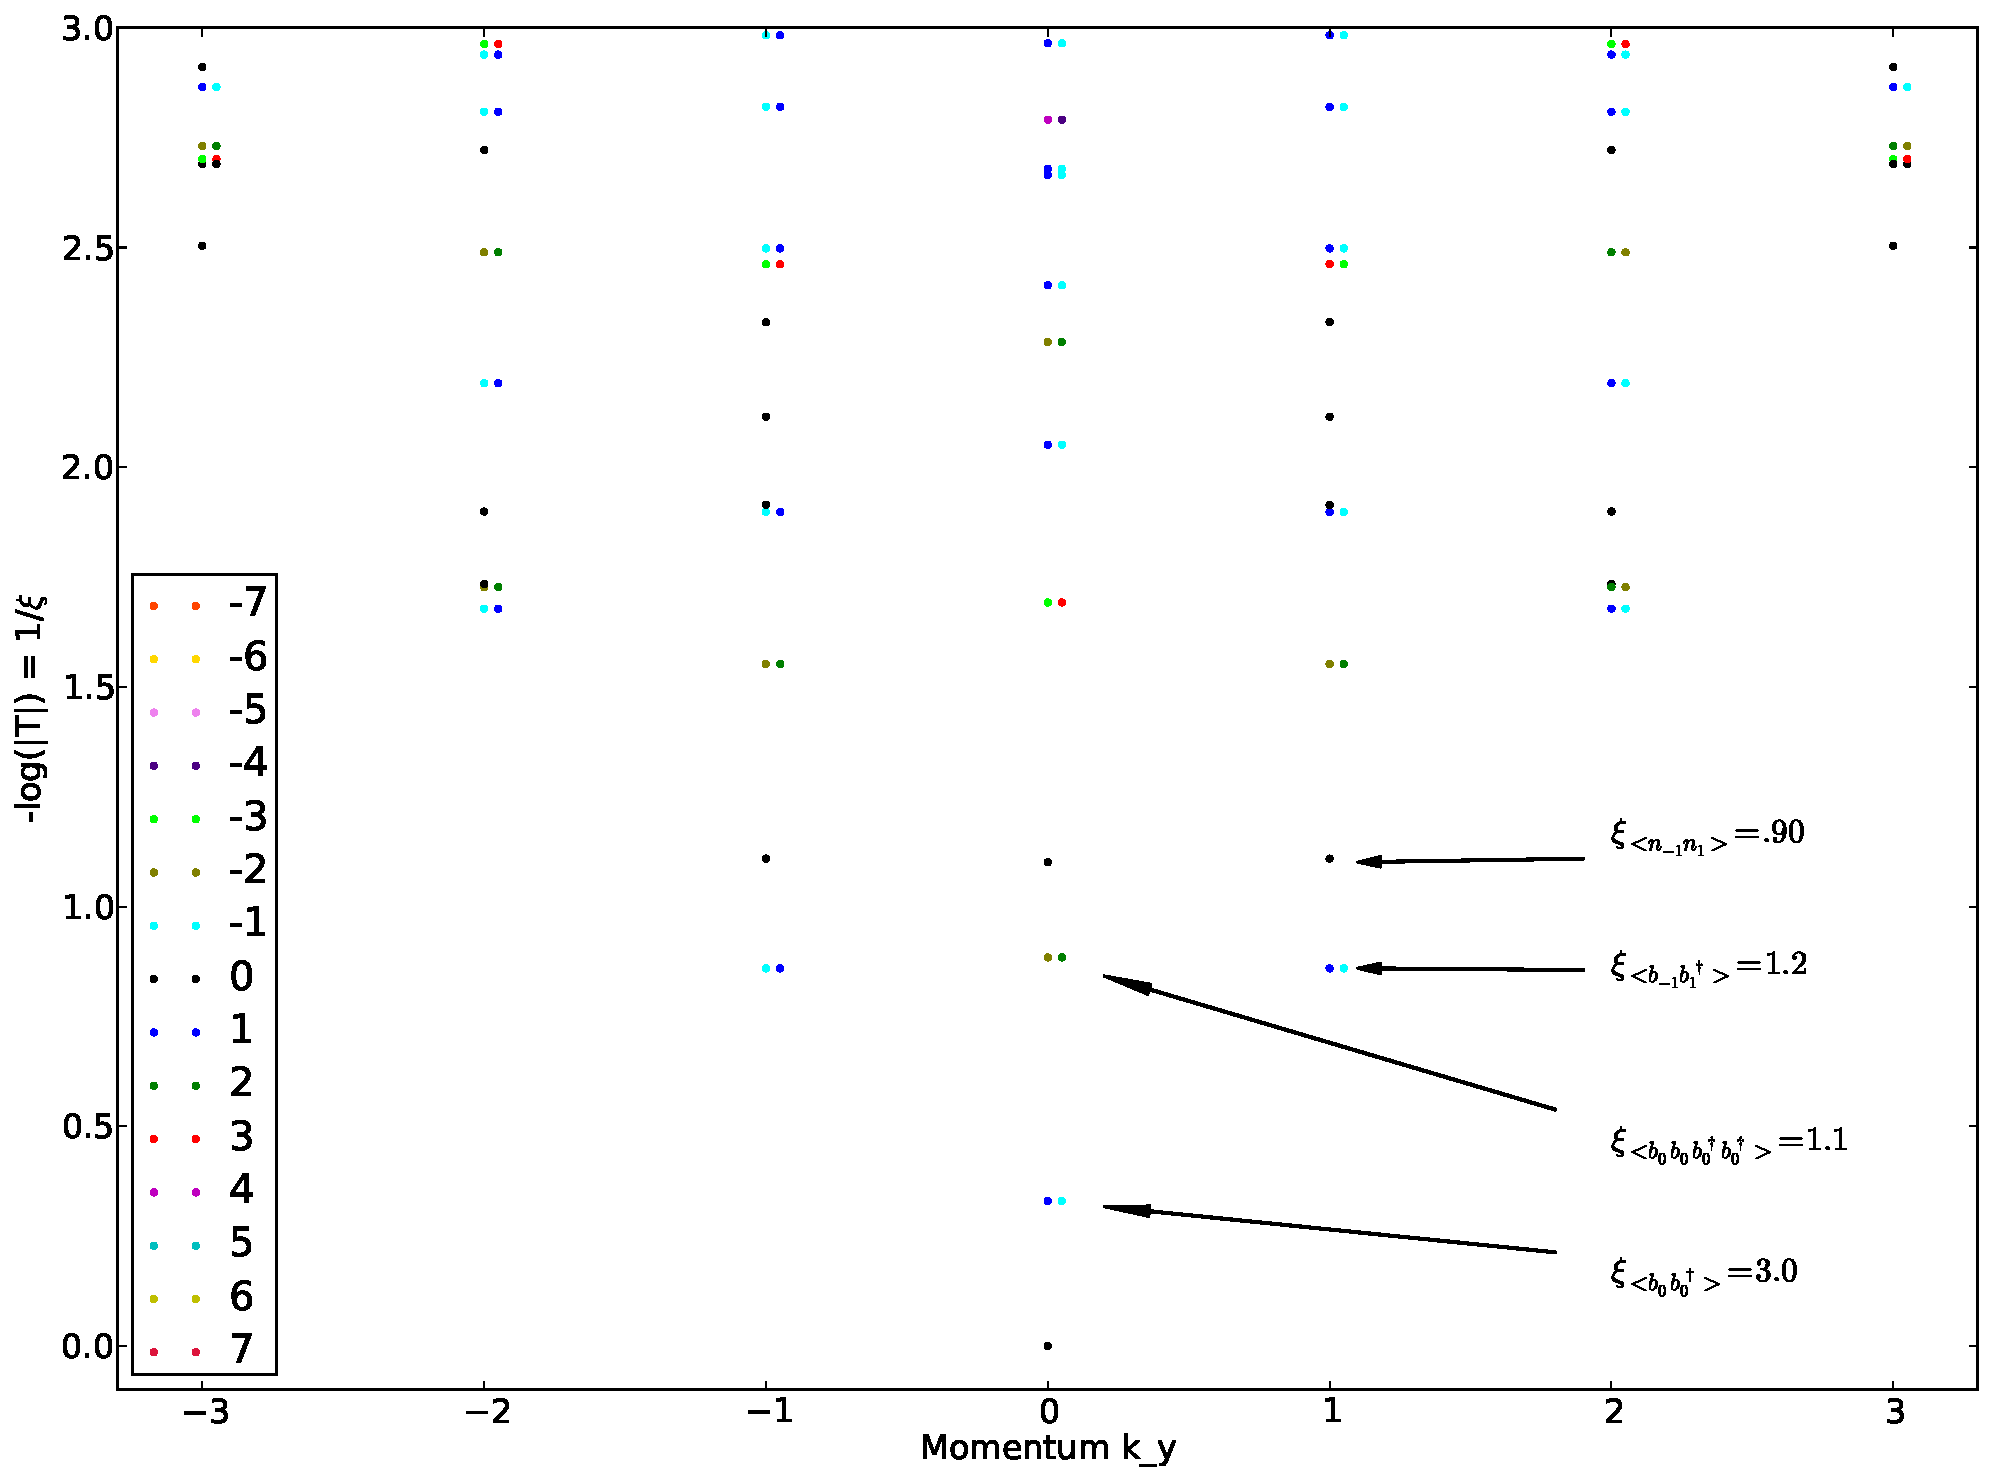
\includegraphics[width=5in, height=3.5in]{{softcoreboson/plots/annotated_L7transfer_matrix_spectrum.pdf}}
\end{center}
\caption{Spectrum of inverse correlation lengths for the soft-core boson state with L = 7. The annotations indicate the spectrum points with the quantum numbers appropriate for the boson correlation function $<b^{\dagger}_k b_{-k}>$ and the density correlation function $<n_{k} n_{-k}>$.}
	\label{fig:scb-tms}
\end{figure}These plots give us a quick way to assess the correlation properties of the proposed bosonic states. However, the information they show is inherently one dimensional - they determine how the correlation functions behave asymptotically as you go down the length of the cylinder, not  how it behaves at short distances or in the circumferential direction. These correlation lengths are subject to large finite size effects in the circumference of the cylinder. Furthermore, operators with the same quantum numbers can't be distinguished without more work.

In the next section, we will look at these transfer matrix spectrum plots and the correlation length bounds that they imply. Section \ref{sec:detailed} will look instead at the more detailed short distance correlation function data. 

\subsection{Correlation Bounds for Bosonic States}

These plots show the lowest spectrum points, which correspond to the heighest weights of the transfer matrix, in more detail. First, the soft-core boson state is shown for multiple cylinder widths. 

\begin{figure}[hbctp]
\includegraphics[width=\textwidth]{{softcoreboson/plots/finite_size_transfer_matrix_spectrum_with_corr2.pdf}}
\caption{Lowest few eigenvalues of the transfer matrix spectrum for soft-core boson state shown for cylinder widths $L=5, 6, 7, 8$. Color indicates boson number $N$; the degenerate spectum points at negative charge are suppressed from the plot. The data from the lowest non-zero eigenvalue occuring for $K=0, N=1$, and the $K=0, N=0$ eigenvalue are used to make the correlation length bounds shown on the right. Finite size extrapolation predicts that the correlation bound for all sectors is around $3.2$, and for symmetric sectors is around $1.7$, using a decaying exponential fit - but significant finite-size effects exist.
}
\label{fig:scb-tms-fs}
\end{figure}

It is clear from this data that the overall correlation length bound has a finite limit, and thus all correlation functions will be gapped. 
Attempting to fit power law or logarithmically increasing functions to the correlation length data does not give good results, while the exponentially decaying fit function shown in Figure \ref{fig:scb-tms-fs} fits well. 

On the other hand, if we had found that the decay constants of the exponentials decreased to zero as the MPS bond-dimension increased, it could be that the actual correlation functions show power-law decay in the thermodynamic limit of an infinitely wide cylinder. This could not occur for a MPS product state limited to a fixed bond dimension, but it can occur for a PEPS with a finite-bond dimension, given the effective MPS bond dimension that grows with the circumference of the cylinder. Thus, a PEPS can represent a critical point with finite bond dimension, with the infinite correlation length detectable using finite-size scaling.

Given the strong finite-size corrections that appear - especially for the symmetric sector - the extrapolated correlation lengths shouldn't be taken as exact, just indicative of greater or less correlations.

\begin{figure}[hbctp]
\includegraphics[width=\textwidth]{{hardcoreboson/plots/finite_size_transfer_matrix_spectrum_with_corr2.pdf}}
\caption{Same as Figure \ref{fig:scb-tms-fs} but with the hard-core boson state instead. Finite size extrapolation shows that the correlation length bound for all sectors is around $8.4$, and for symmetric sectors is around $3.6$. Note the increase of correlation length over the soft-core boson states, as well as the increase in finite-size corrections.
}
	\label{fig:hcb-tms-fs}
\end{figure}

The hard-core boson states had much larger correlations than the soft-core states, as shown in Figure \ref{fig:hcb-tms-fs}. This may be unexpected. Applying the hard-core projection suppresses boson-number fluctuations, so naively it should move you further from the phase-transition to a superfluid, where boson-number fluctuations diverge.



This increase in correlations could be explained if applying the hard-core projection causes the system to pass through a phase transition. By continuously tuning the PEPS parameters $b_1, b_2$ from the soft-core state with $b_1 = b_2 = 1$ to the hard-core state with $b_1 = b_2 = 0$, we found that the correlation length increases monotonically from the soft-core state to the hard-core state, as shown in Figure \ref{fig:scb-to-hcb-tuning}. This seems to rule out a phase transition as the explanation for the increase in correlations.


\begin{figure}[hbctp]
\begin{center}
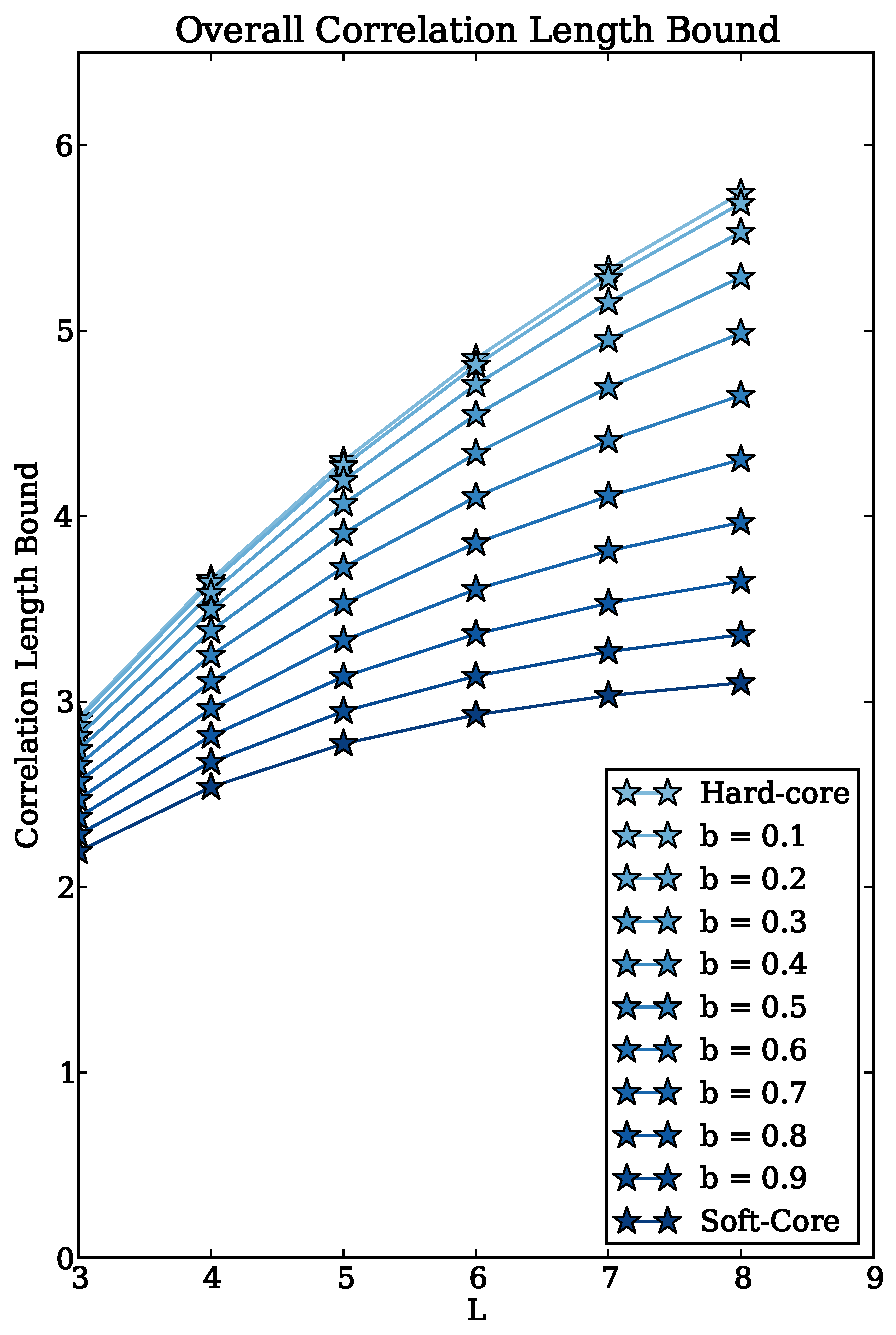
\includegraphics[width=0.5\textwidth]{{interpolatedboson/plots/Overall_Correlation_Length.pdf}}
\end{center}
\caption{Correlation length bound when the PEPS parameters are tuned from the soft-core to the hard-core boson states along the line $b_1 = b_2 = b$. Correlation length monotonically increases as hard-core projection is applied.}
\label{fig:scb-to-hcb-tuning}
\end{figure}
\subsection{Detailed Correlation Functions}
\label{sec:detailed}
Using Equation (\ref{eq:corr}), the computed boson correlator $<b_x b^{\dagger}_0>$ and the density correlator $<n_x n_0>$ are shown in  Figures \ref{fig:scb-bbdagmap}, \ref{fig:scb-nnmap}, \ref{fig:hcb-bbdagmap}, and \ref{fig:hcb-nnmap} in the Appendix.

The correlation maps confirm properties of the correlation functions predicted by the transfer matrix spectrum alone: that the correlation lengths increase with cylinder circumference $L$, that they increase as you tune from the the soft-core to the hard-core state, and that the density-density correlations are much more short-ranged than the hopping correlation functions. 

While the correlation length determined from the asymptotic decay of the hopping is greater in the hard-core state in comparison to the soft-core state, the short distance hopping is actually much smaller. This short distance hopping is suppressed by the hard-core projection due to the lack of available states to hop into when neighboring sites are filled.  

Another notable feature here is that the full point group symmetry of the honeycomb lattice is recovered at short distances in the correlation functions, despite not being a symmetry of the honeycomb on a cylinder due to the periodic boundary conditions. If the state spontaneously breaks rotational symmetry in the thermodynamic limit, we would expect to instead see sensitivity to the boundary conditions at finite sizes.

The correlation functions are shown plotted versus distance along the cylinder in Figure \ref{fig:bdagb-scatter}. The minimum distance $d(x)$ along the cylinder for the points reachable by $x$ applications of the transfer matrix is asymptotically $d(x) \approx 1.5x$, so one would expect the correlation length measured along the cylinder to be around $1.5$ times the MPS correlation length. 
\begin{figure}[hbctp]
\begin{center}
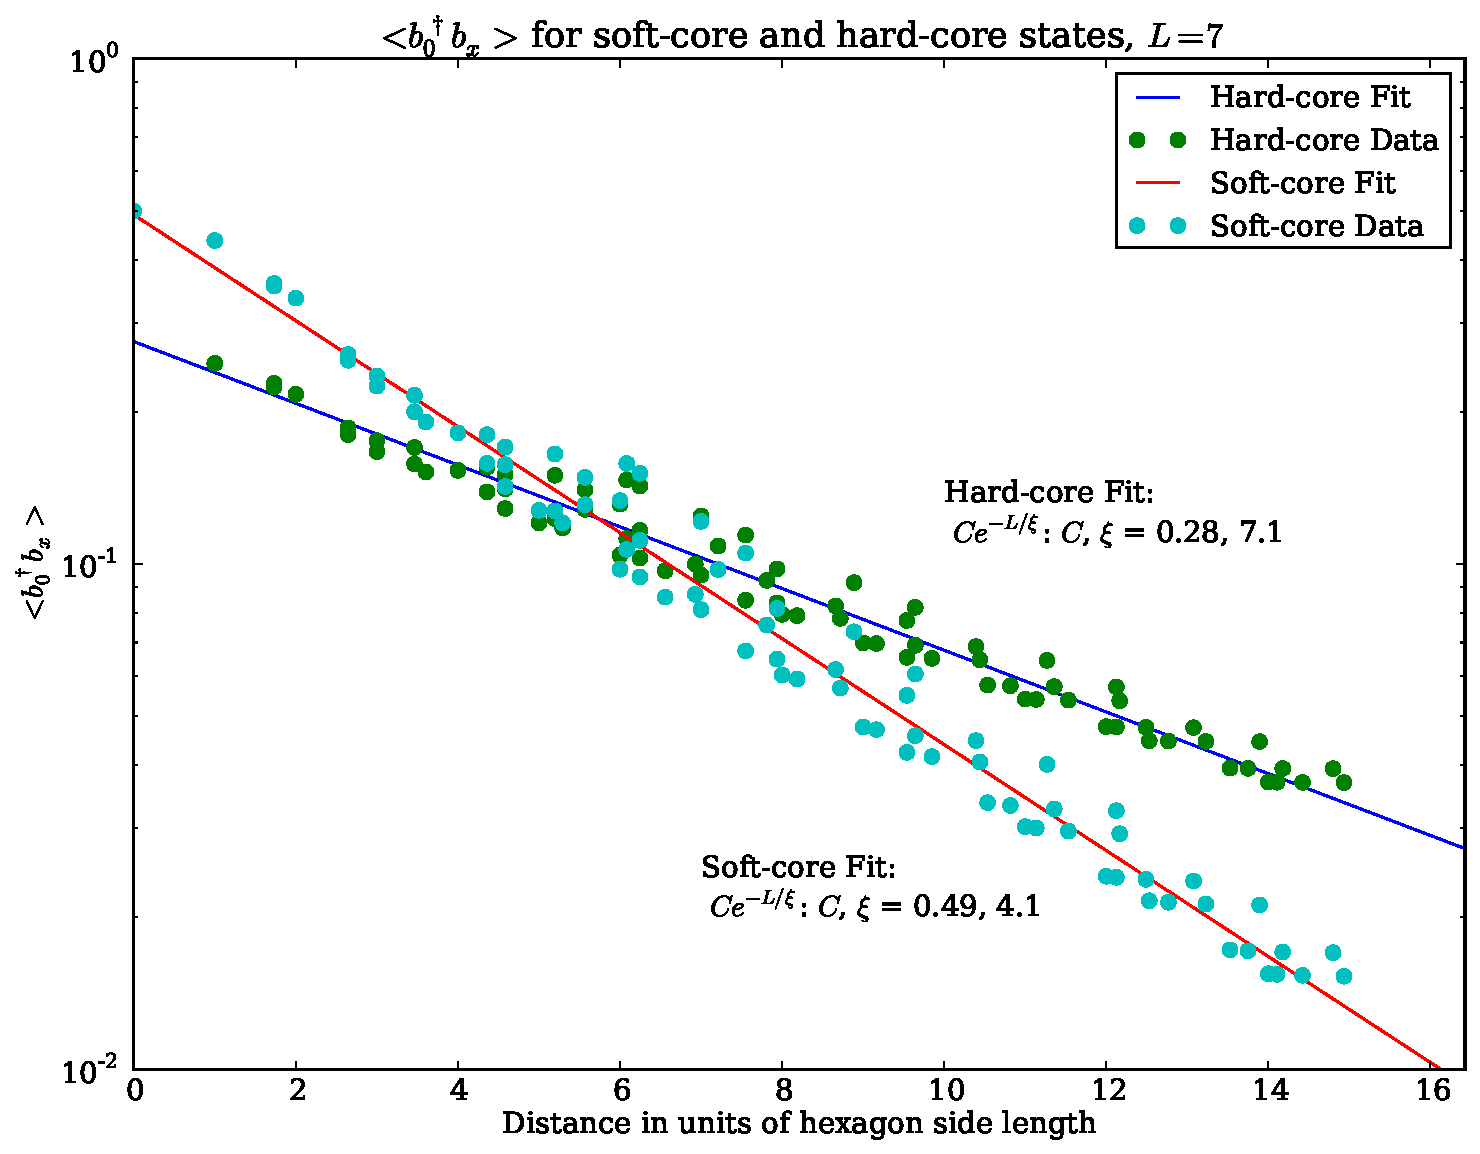
\includegraphics[width=6in]{{summary/log_bdagb_corr_comparison.pdf}}
\end{center}
\caption{The correlation function $<b_x b^{\dagger}_0>$ shown on a log-scale for the hard-core and soft-core boson states. The distance $d_x$ is computed using the shortest path along the cylinder and measured in units of the hexagon side length. Compare to the MPS correlation length 3.0 for the soft-core boson and 5.4 for the hard-core boson at $L=7$.}
	\label{fig:bdagb-scatter}
\end{figure}

\begin{figure}[hbctp]
\begin{center}
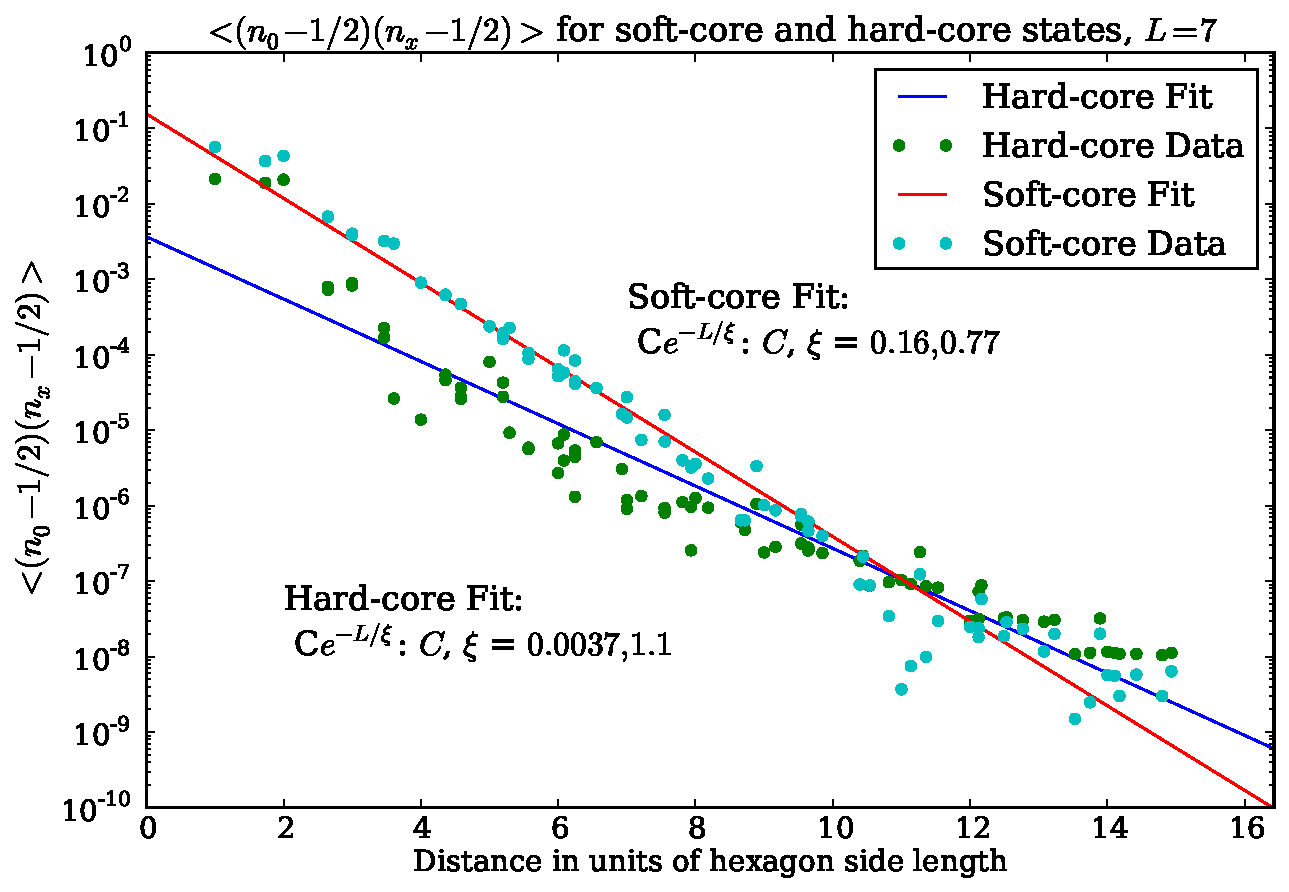
\includegraphics[width=6in]{{summary/log_nn_corr_comparison_abs3.pdf}}
\end{center}
\caption{The absolute value of the connected density correlation function $|<(n_x - \frac{1}{2})(n_0 - \frac{1}{2})>|$ shown on a log-scale for the hard-core and soft-core boson states. The correlation values are both positive and negative - an alternate version of this plot that shows the sign structure is in Figure \ref{fig:signed-nn-scatter}. Compare to the symmetric MPS correlation length 0.9 for the soft-core boson and 1.1 for the hard-core boson at $L=7$.}
	\label{fig:nn-scatter}
\end{figure}

\subsection{Entanglement properties of the boson states}

The eigenvector $\vket{v}_B$ (and similarly the left eigenvector $\vbra{v}_A$) of the transfer matrix represents a density operator $\rho_{B}$ on the Hilbert space of the virtual qubits at the right edge (left edge) of a half-infinite cylinder. ($\rho_{B}$ is formed by reshaping $\vket{v}_B$.) The spectrum of this density operator coincides with the reduced density matrix formed from the wavefunction on a fully infinite cylinder and tracing over all the degrees of freedom on half the cylinder. \cite{Ignacio_Cirac2011-te}

This density matrix $\rho_{B}$ is Hermitian, positive semidefinite, and can be rescaled to have trace 1. It is also block-diagonal in the appropriate basis of boson number and transverse momentum eigenstates. The operator $H_e$ satisfing $\rho_{B} = \exp{-H_e}$ is called the entanglement Hamiltonian, and its spectrum the entanglement spectrum. 
These spectra can be used to characterize long-range entanglement properties in the states. In particular, topological order can sometimes be identified by a gapless spectrum and non-zero topological entanglement entropy, 
and symmetry protected topological order can sometimes be identified by a gapless spectrum appearing only if the entanglement cut respects the symmetry.%citation needed%

Full entanglement spectra for the soft-core state is shown in Figures \ref{fig:sc-entanglement-spectrum} and \ref{fig:hc-entanglement-spectrum}. 

The states satisfy the expected area law scaling for entanglement entropy, that is the entanglement entropy is linear in the cylinder circumference, as shown in Figure \ref{fig:entanglement-entropy}. These plots also show that the topological entanglement entropy, defined via the subleading constant correction to the area law, is 0. 
\begin{figure}[hbctp]
\centering
\begin{minipage}{.5\linewidth}
  \centering
  \includegraphics[width=\linewidth]{summary/sc-entanglement_entropy_L8.png}
  %\captionof{figure}{A figure}
  %\label{fig:test1}
\end{minipage}%
\begin{minipage}{.5\linewidth}
  \centering
  \includegraphics[width=\linewidth]{summary/hc-entanglement_entropy_L8.png}
  %\captionof{figure}{Another figure}
  %\label{fig:test2}
\end{minipage}
\caption{Entanglement entropy for soft-core (left) and hard-core (right) states. The topological correction to area-law scaling is consistent with 0.}
\label{fig:entanglement-entropy}
\end{figure}


By careful finite-size analysis of the low-energy entanglement spectrum of the soft-core boson state, we find that the spectrum can be consistently matched to the gapless spectrum of a compactified free boson, a CFT with central charge $c = 1$; however, complicating factors eliminate the possibility of seeing the characteristic degeneracy patterns and $\frac{1}{L}$ finite-size scaling that would be the most convincing evidence of this identification. These spectrum patterns appear when comparing shifted, rescaled entanglement energies over several system sizes, as detailed in Figure \ref{fig:sc-scaled-entanglement-spectrum}.

\begin{figure}[hbctp]
\begin{center}
\includegraphics[width=\textwidth]{{softcoreboson/plots/scaled_entanglement_spectraL9.pdf}}
\end{center}
\caption{Rescaled entanglement spectrum for the soft-core boson state on the zig-zag edge cylinder, for system sizes $L=5, 6, 7, 8,$ and $9$ (from left to right). The energy scale is set by the energy difference between the lowest two states with boson-number $N = 1$. A chemical potential term $-\mu N$ is added to shift the lowest boson-number energy to 1. This fixes the lowest three points in the spectrum, marked by lines. These transformations remove most of the system size dependence for the lowest energy points in the boson-number $N=2, 3, 4$ sectors as well, and the energies of those points appears to be a quadratic function of $N$, as shown in Figure \ref{fig:determiningK}. This fact and the approximate degeneracies of $1, 1, 2, 3$ in the $N=3$ sector suggest a description by a free-boson CFT.}
\label{fig:sc-scaled-entanglement-spectrum}
\end{figure} 

Given the $U(1)$ symmetry of the state, the simplest possible conformal field theory we might expect to appear at the edge is that of a single free bosonic field. We cannot use the ground-state of the entanglement Hamiltonian to compute the central charge, as the appropriate charge 0 symmetry sector is represented only by a single state in our edge Hilbert space - the ground-state wavefunction is just $\ket{000...0}$. For the same reason, we cannot expect to identify the characteristic degeneracy pattern of descendant states in the spectrum. We'll have to rely instead on a comparison of the actual energy values to test whether the free boson CFT is an appropriate match.

The free-boson CFT is created from the Lagrangian 
$$ \mathfrak{L} = \frac{g}{2}\int dt \int\limits_0^L dx ( \frac{1}{v^2}(\partial_t \phi)^2 - (\partial_x \phi)^2)$$
and with the compatified field identification
$$ \phi \equiv \phi + 2\pi R$$
and placed on the circle of circumference $L$ with periodic boundary conditions
$$ \phi(x) \equiv \phi(x+L).$$

After canonical quantization, it is found that the set of energy eigenstates consists of $U(1)$ Kac-Moody primaries $\ket{e, m}$, with integers $e, m$ labeling the $U(1)$ charge and the winding number of the bosonic field respectively, and level $n, \bar{n}$ descendant fields $\mathbf{\bar{j}}_{-\bar{n}} \mathbf{j}_{-n} \ket{e, m}$ with nonnegative integers $n, \bar{n}$. The properties of the $U(1)$ Kac-Moody algebras constrain the form of energy and momentum eigenvalues - for the state $\mathbf{\bar{j}}_{-\bar{n}} \mathbf{j}_{-n} \ket{e, m}$, 

\begin{eqnarray*}
\text{the eigenvalue of }
&\mathbf{L_0}& \text{ is } \frac{1}{2}(Ke + \frac{m}{K})^2 + n\text{,}\\
&\mathbf{\bar{L}_0}& \text{ is } \frac{1}{2}(Ke - \frac{m}{K})^2 + \bar{n}\text{,}\\
&\mathbf{P}& = \mathbf{L_0} - \mathbf{\bar{L}_0} \text{ is } em + n - \bar{n}\text{,}\\
&\mathbf{H}& = \mathbf{L_0} + \mathbf{\bar{L}_0} \text{ is } K e^2 + \frac{1}{K}m^2 + n + \bar{n}
\label{eq:spectrum}
\end{eqnarray*}

Momentum is a good quantum number due to the periodic boundary conditions, and the allowed values are integer multiples of $2\pi /L$, with the integer given by the eigenvalue of $\mathbf{P}$. It is this integer that is used as momentum in all of the spectrum plots.

After rescaling and setting the velocity $v$ to $1$, only the dimensionless parameter $K = 2 \pi g R^2$, called the Luttinger parameter, appears in the energy eigenvalue $H$. (Note: the spectrum is unchanged by the duality relation $K \rightarrow \frac{1}{K}, e \leftrightarrow m$.) The scaling with system size of all of the energy eigenvalues is $1/L$. 

A generic Hamiltonian in the phase of the bosonic CFT will have this spectrum complicated by couplings to irrelevant operators, which destroy the pattern for high-energy states, by couplings to marginal operators, which renormalize the value of $K$ and add logarithmic finite-size corrections, and additionally by a chemical potential term $-\mu \mathbf{N}$, where $N$ is the boson number. 

Therefore, to compare the spectrum of the density matrix to the CFT spectrum, we will need to restrict to low energy states, shift the lowest energy to 0, rescale the velocity to 1, and add a boson-number dependent shift of the form $\mu N$. As shown in Figure \ref{fig:sc-scaled-entanglement-spectrum}, this procedure results in a few energy eigenvalues not fixed by this procedure that appear approximately constant from system sizes $L=5$ to $L=8$, in particular the lowest energy state from the sectors with boson-number 2, 3, and 4. These would correspond to the states with $m=n=\bar{n}=0$, $e = 2, 3, 4$, and energy $H = Ke^2 + \mu e$. Fixing the energy of the state $e=1, m=n=\bar{n} = 0$ to $1$ by adding a chemical potential term leads to the form $H = Ke^2 + (1 - K)e$. In Figure \ref{fig:determiningK}, we see that this is indeed a good way of describing the energies for these states.


\begin{figure}[hbctp]
\begin{center}
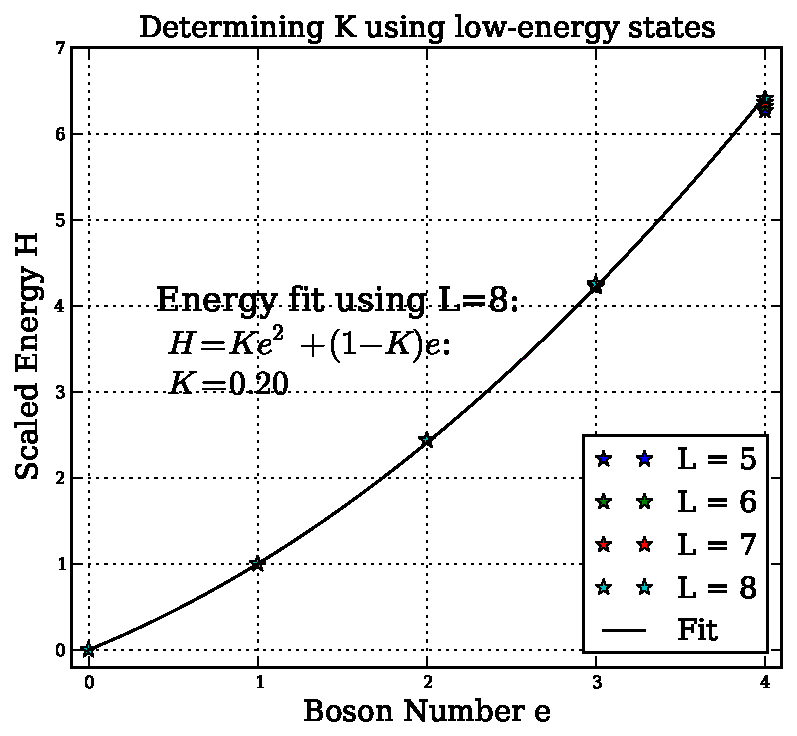
\includegraphics[width=4in]{{summary/determining_K.pdf}}
\end{center}
\caption{The energies for the lowest state in the boson number sector $e$ using the values from Figure \ref{fig:sc-scaled-entanglement-spectrum} are found to be a quadratic function of $e$, as in the CFT of a free boson. The values at $e = 0, 1$ are fixed to $0, 1$, and the others fit to the form $H = Ke^2 + (1 - K)e$. The fit is good with the quadratic coefficent $K=0.2$ at $L=8$, with other system sizes nearly the same.}
	\label{fig:determiningK}
\end{figure}  

In addition, the bosonic CFT predicts that the state $ \mathbf{j}_{-n} \ket{e, m}$ is degenerate with the states $$ \mathbf{j}_{-1}^n \ket{e, m}, \mathbf{j}_{-1}^{n-2} \mathbf{j}_{-2} \ket{e, m}, ... \prod\limits_{i=1}^{\infty} \mathbf{j}_{-i}^{n_i} $$ where the total level is  $$\sum\limits_{i=1}^{\infty} i*n_i = n$$. 
This leads to a total degeneracy of $Z(n)*Z(\bar{n})$ for the state $\mathbf{\bar{j}}_{-\bar{n}} \mathbf{j}_{-n} \ket{e, m}$ where $Z(n)$ is the number of partitions of the integer $n$. In particular, for chiral descendents with $\bar{n} = 0$, the first few degeneracies are $Z(n) = 1, 1, 2, 3$ for $n = 0, 1, 2, 3$. Although it is impossible for the charge 0 or 1 states on this edge Hilbert space to contain the predicted degeneracy, the lowest charge 2 states at momenta $p = 0, 1, 2$ and the lowest charge 3 states at momenta $p=0, 1, 2, 3$ do show approximate degeneracies that match this pattern. A tentative identification of these descendant states is shown in Figure \ref{fig:spec-id}.


\begin{figure}[hbctp]
\begin{center}
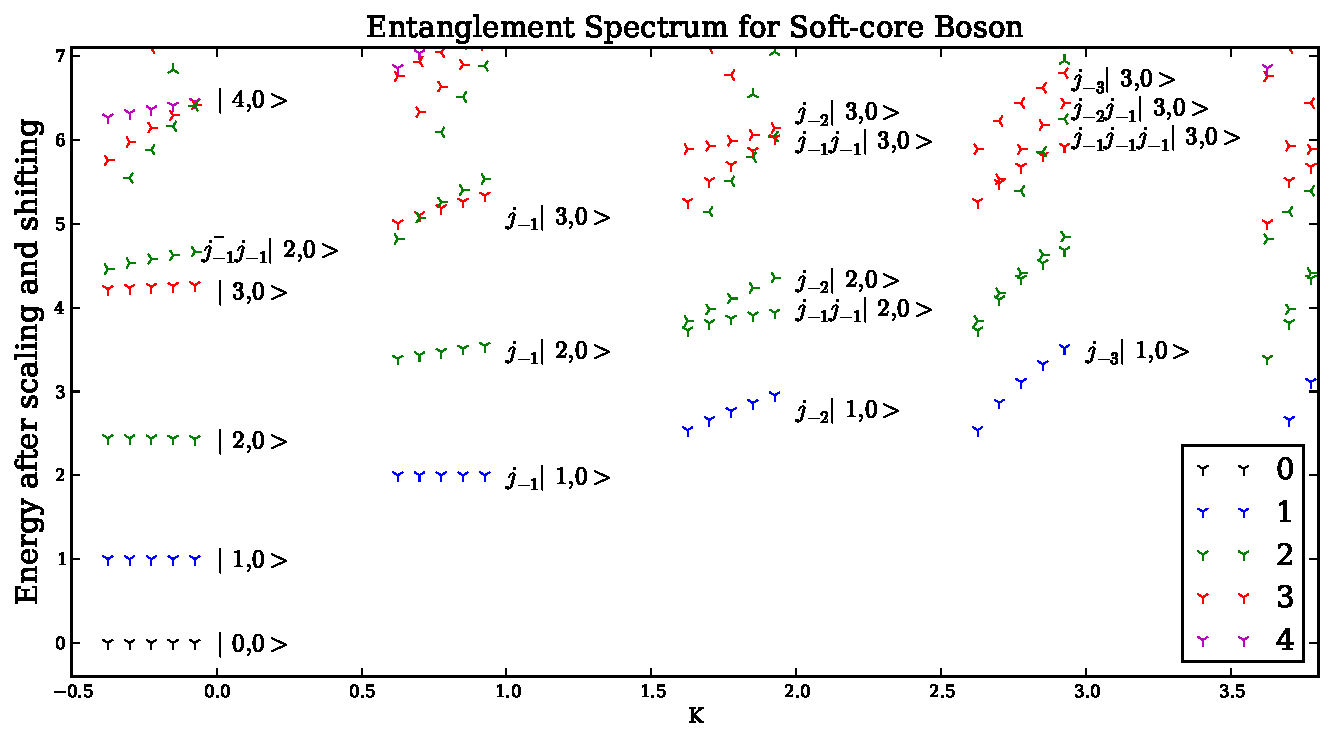
\includegraphics[width=6in]{{summary/sc-spectrum-id.pdf}}
\end{center}
\caption{The soft-core entanglement spectrum with the matching bosonic CFT states. The degenerate states at each level will potentially mix.}
	\label{fig:spec-id}
\end{figure}  

For the hard-core boson state, the entanglement spectrum is very nearly described by the soft-core spectrum with a chemical potential shift large enough to change the ground state. The hard-core spectrum before and after shifting the chemical potential can be seen in Figures \ref{fig:hc-scaled-entanglement-spectrum2} and \ref{fig:hc-scaled-entanglement-spectrum3}. The energies for the lowest state in the boson number sector $e$ are still quadratic, and with the same value of the quadratic coefficient $K$, $K \approx 0.2$. The similarity of the spectra in Figures \ref{fig:sc-scaled-entanglement-spectrum} and \ref{fig:hc-scaled-entanglement-spectrum3} supports the conclusion that no phase transition occurs as the hard-core projection is applied continuously, although in general adding an interaction could change the value of $K$. 

\begin{figure}[hbctp]
\begin{center}
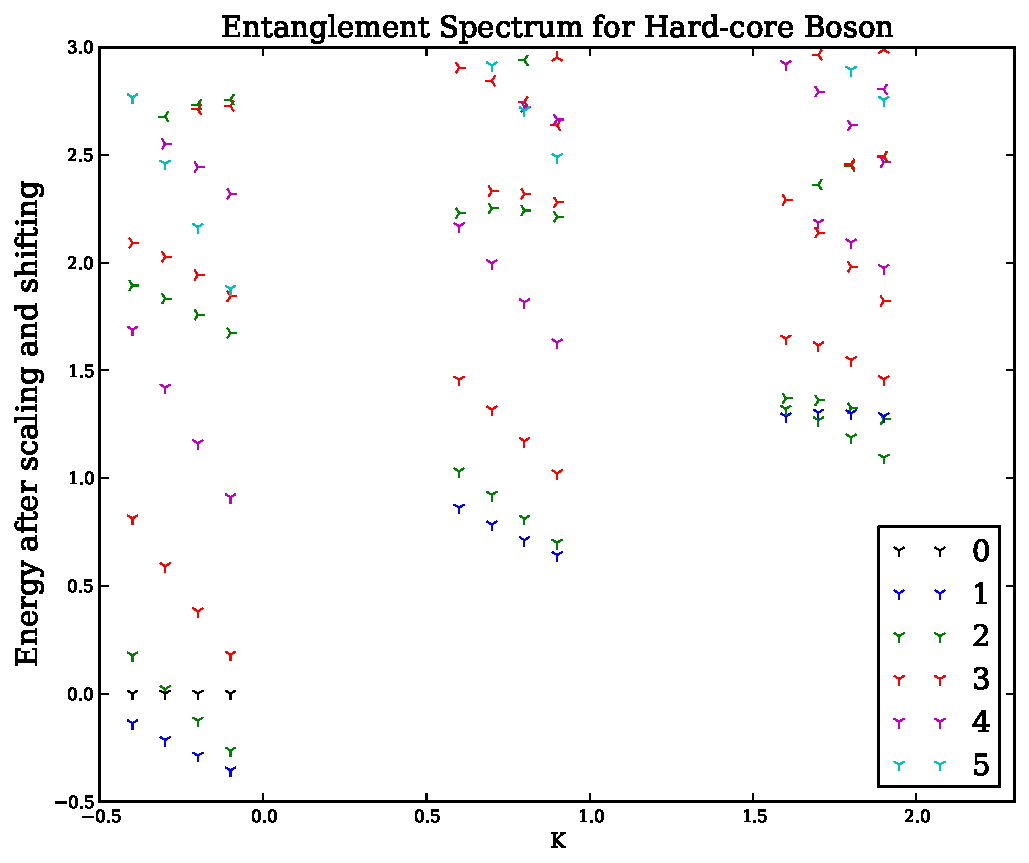
\includegraphics[width=\textwidth]{{hardcoreboson/plots/scaled-entanglement-spectra2.pdf}}
\end{center}
\caption{Rescaled entanglement spectrum for the hard-core boson state on the zig-zag edge cylinder, for system sizes $L=5, 6, 7,$ and $8$ (from left to right). The energy scale is set by the energy difference between the lowest two states with boson-number $N = 1$, and the zero of energy is fixed by the single charge 0 state. No chemical potential shift has been added yet.}
\label{fig:hc-scaled-entanglement-spectrum2}
\end{figure} 

\begin{figure}[hbctp]
\begin{center}
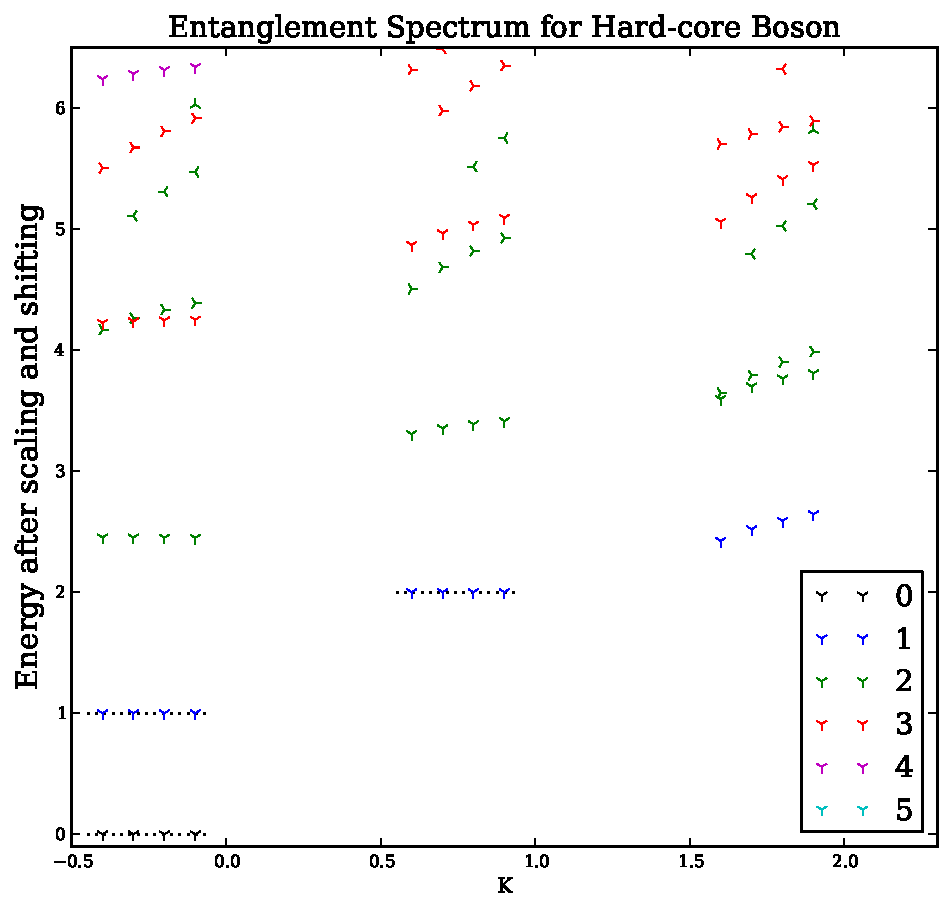
\includegraphics[width=\textwidth]{{hardcoreboson/plots/scaled-entanglement-spectra3.pdf}}
\end{center}
\caption{Rescaled entanglement spectrum for the hard-core boson state on the zig-zag edge cylinder, for system sizes $L=5, 6, 7,$ and $8$ (from left to right). The energy scale is set by the energy difference between the lowest two states with boson-number $N = 1$, and the zero of energy is fixed by the single charge 0 state. A chemical potential shift has been added to fix the charge 1 ground state to energy 1. The spectrum is nearly identical to the soft-core boson spectrum at this point.}
\label{fig:hc-scaled-entanglement-spectrum3}
\end{figure} 

\begin{figure}[hbctp]
\begin{center}
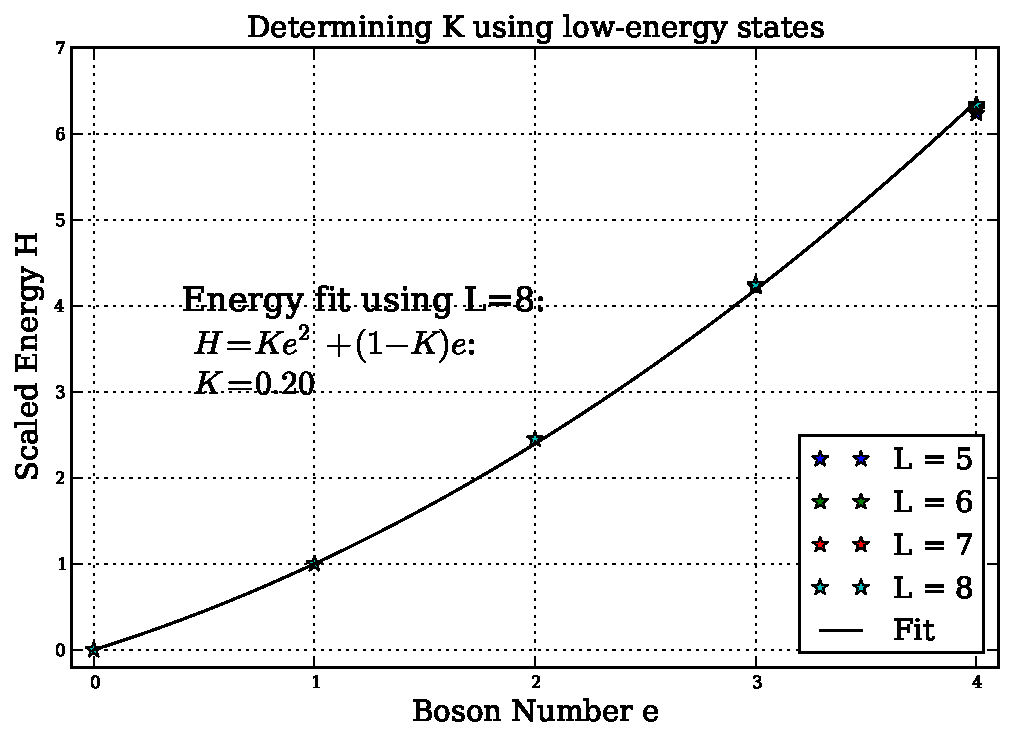
\includegraphics[width=6in]{{summary/hc-determining_K.pdf}}
\end{center}
\caption{The hard-core boson version of Figure \ref{fig:determiningK}. The energies for the lowest state in the boson number sector $e$ using the values from Figure \ref{fig:hc-scaled-entanglement-spectrum3} are found to be a quadratic function of $e$, as in the CFT of a free boson, with the quadratic coefficent $K=0.2$ at $L=8$.}
	\label{fig:hc-determiningK}
\end{figure}  

\newpage
\subsection{Comparision with other entanglement cuts}

In order to test the hypothesis that this 'gapless' entanglement edge is protected by lattice symmetries, we can explicitly break the symmetry or choose an entanglement cut that respects a different subset of the honeycomb space group. 

In particular, if we can put the honeycomb lattice on a cylinder, we explicitly break all of the point group symmetry besides the reflections across axes parallel to the periodic identification. If the honeycomb was on the cylinder in the zig-zag configuration, there is a simple entanglement cut that respects the remaining reflection symmetry. For the armchair configuration, there is no such cut. 

The entanglement spectrum for the soft-core boson state in the armchair configuration with the cut is shown in Figure \ref{fig:armchair-entanglement-spectrumL3} with $L=6$ sites. Note that translation symmetries on this edge shift by multiples of 2 sites, so only three momentum eigenvalues are available. We find that despite the symmetry breaking, the entanglement spectra can still be described by the same pattern as in Figure \ref{fig:sc-scaled-entanglement-spectrum} after shifting the chemical potential. (To make the Hilbert space comparable, we measure the charge of the edge states relative to the minimum possible charge, as opposed to the natural definition given by the PEPS.) 

\begin{figure}[hbctp]
\begin{center}
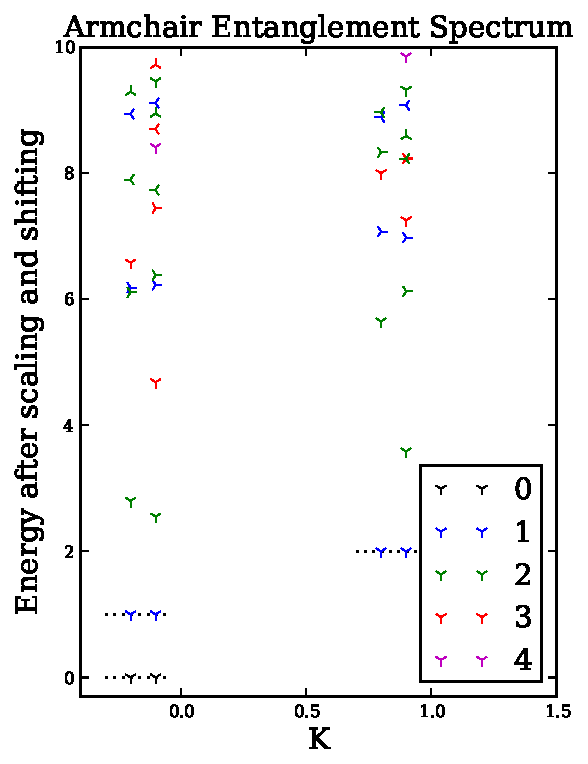
\includegraphics[width=3.5in]{{armchair_softcoreboson/plots/scaled-entanglement-spectrumL23.pdf}}
\end{center}
\caption{Entanglement spectrum for the armchair boson state.  The same pattern from \ref{fig:sc-scaled-entanglement-spectrum} is approximately recovered. In particular, the ground states of the charge 2 and 3 sectors appear around $Ke^2+(1-K)e$ with $K=0.2$ and $e=2, 3$. The points shown correspond to 4 and 6 sites on the edge (2 or 3 edge unit cells), from left to right. The charge shown in the legend (and used to color the points) is measured as a difference from the minimum possible boson number in the edge Hilbert space - i.e. the charge $-3$ ground state of Figure \ref{fig:armchair-entanglement-spectrumL3} is now labeled as charge $0$. There is only one state in that charge sector.}
\label{fig:armchair-entanglement-spectrum}
\end{figure} 

We can also put the PEPS on a zig-zag edge cylinder in a different way than the earlier calculations, by rotating the site tensors. This leads to an exactly equivalent physical wavefunction, but changes the nature of the virtual edges crossed. (Remember, the PEPS breaks the rotational symmetry at the virtual level.) All correlation functions, Schmidt eigenvalues/states, or other quantities defined only in terms of the physical wavefunction should come out the same. The entanglement spectrum can be computed up to $L=5$ using this cut. The entanglement spectrum again gives the same pattern after relabeling charge as the difference from the maximum possible charge, shifting the chemical potential, and rescaling.

\begin{figure}[hbctp]
\begin{center}
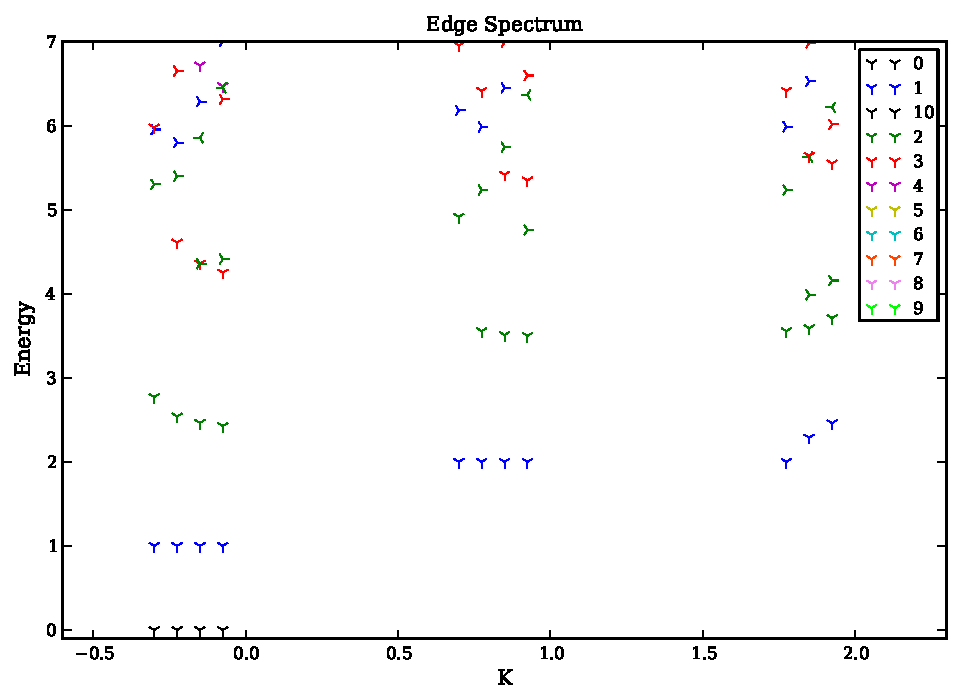
\includegraphics[width=6in]{{rotated_softcoreboson/plots/edge_specL5_u1numshift_mushift.pdf}}
\end{center}
\caption{Entanglement spectrum for the rotated cut on the soft-core boson state.  The same pattern from \ref{fig:sc-scaled-entanglement-spectrum} is approximately recovered. In particular, the ground states of the charge 2 and 3 sectors appear around $Ke^2+(1-K)e$ with $K=0.2$ and $e=2, 3$. The points shown correspond to 4 and 6 sites on the edge (2 or 3 edge unit cells), from left to right. The charge shown in the legend (and used to color the points) is measured as a difference from the maximum possible boson number in the edge Hilbert space - i.e. the charge $4$ ground state of Figure \ref{fig:rotated-entanglement-spectrumL5} is now labeled as charge $1$.}
\label{fig:rotated-entanglement-spectrum}
\end{figure} 

By starting with the spectrum of the $K=0.2$ free boson, we can recover the entanglement spectrum of any of the entanglement cuts above by shifting by an appropriate (L dependent) entanglement chemical potential and rescaling by an appropriate (L dependent) scale I'll call entanglement temperature. We can use the tensor network to map the virtual edge states into the physical Schmidt states for a half-infinite cylinder. I don't yet know what the entanglement chemical potential and temperature are telling us about the Schmidt states.

%Momentum is a good quantum number due to the periodic boundary conditions, and the allowed values are integer multiples of $2\pi /L$. As written, the energy value of the states $\hat{\bar{j}}_{-\bar{n}} \hat{j}_{-n} \ket{e, m}$ depend on the parameters $g, R, v$ and scale with system size like $1/L$. After an appropriate rescaling and setting the velocity to $1$, the following form can be found for the spectrum points:
%A second complication is the existance of a continuous family of free boson CFTs, commonly parametrized by the compactification radius of the boson $R$ or the Luttinger parameter $K$. The value of $K$ is determined by a not-universal coefficient of a marginal operator that can generically exist for free boson CFTs. In addition, there is a relevant coefficient $mu$, the boson chemical potential, which must be determined to match the spectra. A final complication, also due to the existance of the marginal operator, is that finite size corrections are in general logarithmic instead of the usual $frac{A}{L}+\frac{B}{L^2}+...$. 
%


%\subsection{Symmetry of the PEPS}
%\label{sec:symmetry}
%We saw in the above section that the eigenstates of the transfer matrix operator can be classified in terms of a boson number, i.e. a charge sector for the $U(1)$ symmetry associated with boson number conservation. In order to assign the appropriate charges to these sectors, it is necessary to figure out how the $U(1)$ symmetry is represented on the virtual states of the PEPS, and in particular on the Hilbert space of virtual qubits on the edge of the cylinder. 
%
%...
%
%We see that we can consistently assign representations of the on-site symmetry group to each virtual bond in the PEPS. The PEPS representation respects the $U(1)$ symmetry, and the transfer operator can be block diagonalized.
%
%On the other hand, the point group symmetry of the wavefunction on the honeycomb lattice is not respected by the PEPS representation - a rotation or reflection of the whole honeycomb lattice gives a different, but equivalent, PEPS representation of the wavefunction. This is due entirely to the choice of a not translationally invariant MPS representation of the W-state used in (\ref{eq:PEPS}). In fact, a translationally invariant representation of the W-state exists, ref??, with a large bond dimension. We can conclude that rotationally invariant PEPS tensors can be acheived, but only with much larger bond dimensions. However, the wavefunction, as well as all physical observables, like correlation functions, will respect the point group symmetry of the underlying lattice.
%
%The honeycomb lattice on the cylinder does not respect the full point group symmetry $D_6$ of the planar honeycomb lattice, but only the reflections with respect to an axis parallel to the period of the cylinder.
%

%
%\subsection{Injectivity of the PEPS}
%\label{sec:injectivity}
%a
\newpage
\section{Appendix - Additional Figures}
\label{sec:Appendix}

\begin{figure}[hbctp]
\centering
 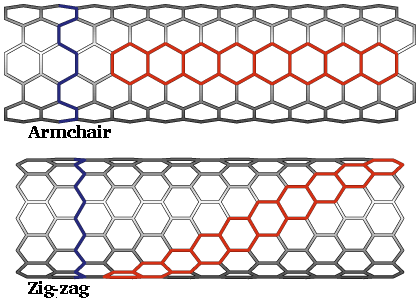
\includegraphics[height=2in, width = 3in]{Zig_Arm.png}
\caption{Zig-zag and armchair configurations of the honeycomb lattice on a cylinder}
%picture source http://phycomp.technion.ac.il/~talimu/structure.html
\label{fig:ZigArm}
\end{figure}



The below figures show the correlation functions for the soft-core and hard-core boson states, on a cylindrical honeycomb lattice in the zig-zag configuration, with circumference $L = 7$. See Figures \ref{fig:ZigArm} and \ref{fig:distances}.

\begin{figure}[hbctp]
\begin{center}
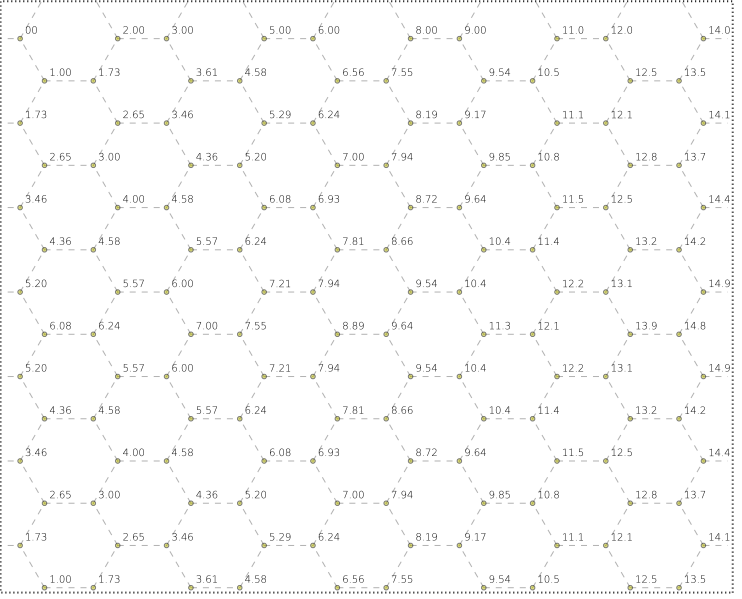
\includegraphics[height=3.7in, width=\textwidth]{{summary/honeycomb_distances2.png}}
\end{center}
\caption{The zig-zag configuration used for the detailed correlation scatter plots below. Values are distances measured along the cylinder, using the shortest path and periodic boundary conditions in the y-direction.}
	\label{fig:distances}
\end{figure}

\begin{figure}[hbctp]
\begin{center}
\includegraphics[width=1\textwidth]{{softcoreboson/L7K0N0/b_xbdag_A0map_try2.pdf}}
\caption{$<b_x b^{\dagger}_0>$ for soft-core boson state with $L = 7$. The subscripts $0$, $x$ refer to the position of the operators, with $0$ being the site in the top-left corner. The correlation function approximately obeys rotational symmetry near the top-left site, despite boundary conditions that don't obey the rotational symmetry.}
\label{fig:scb-bbdagmap}
\end{center}
\end{figure}

\begin{figure}[hbctp]
\begin{center}
\includegraphics[width=\textwidth]{{softcoreboson/L7K0N0/n_xn_A0map_try2.pdf}}
\caption{$<n_x n_0>$ for soft-core boson state with $L = 7$. Due to the average boson density of $\frac{1}{2}$, the density-density correlation function asymptotes to $\frac{1}{4}$. The fluctuations around that mean decay very quickly.}
\label{fig:scb-nnmap}
\end{center}
\end{figure}

\begin{figure}[hbctp]
\begin{center}
\includegraphics[width=\textwidth]{{hardcoreboson/L7K0N0/b_xbdag_A0map_try2.pdf}}
\caption{$<b_x b^{\dagger}_0>$ for hard-core boson state with $L = 7$. Compared to the soft-core boson state, short distance correlation values are less. The hard-core projection reduces the hopping amplitude due to the lack of available states to hop to if neighboring sites are filled. However, asymptotic decay of hopping is slower as you go down the cylinder, consistent with the increased MPS correlation length bound.}
\label{fig:hcb-bbdagmap}
\end{center}
\end{figure}



\begin{figure}[hbctp]
\begin{center}
\includegraphics[width=\textwidth]{{hardcoreboson/L7K0N0/n_xn_A0map_try2.pdf}}
\caption{$<n_x n_0>$ for hard-core boson state with $L = 7$. }
\label{fig:hcb-nnmap}
\end{center}
\end{figure}

\begin{figure}[hbctp]
\begin{center}
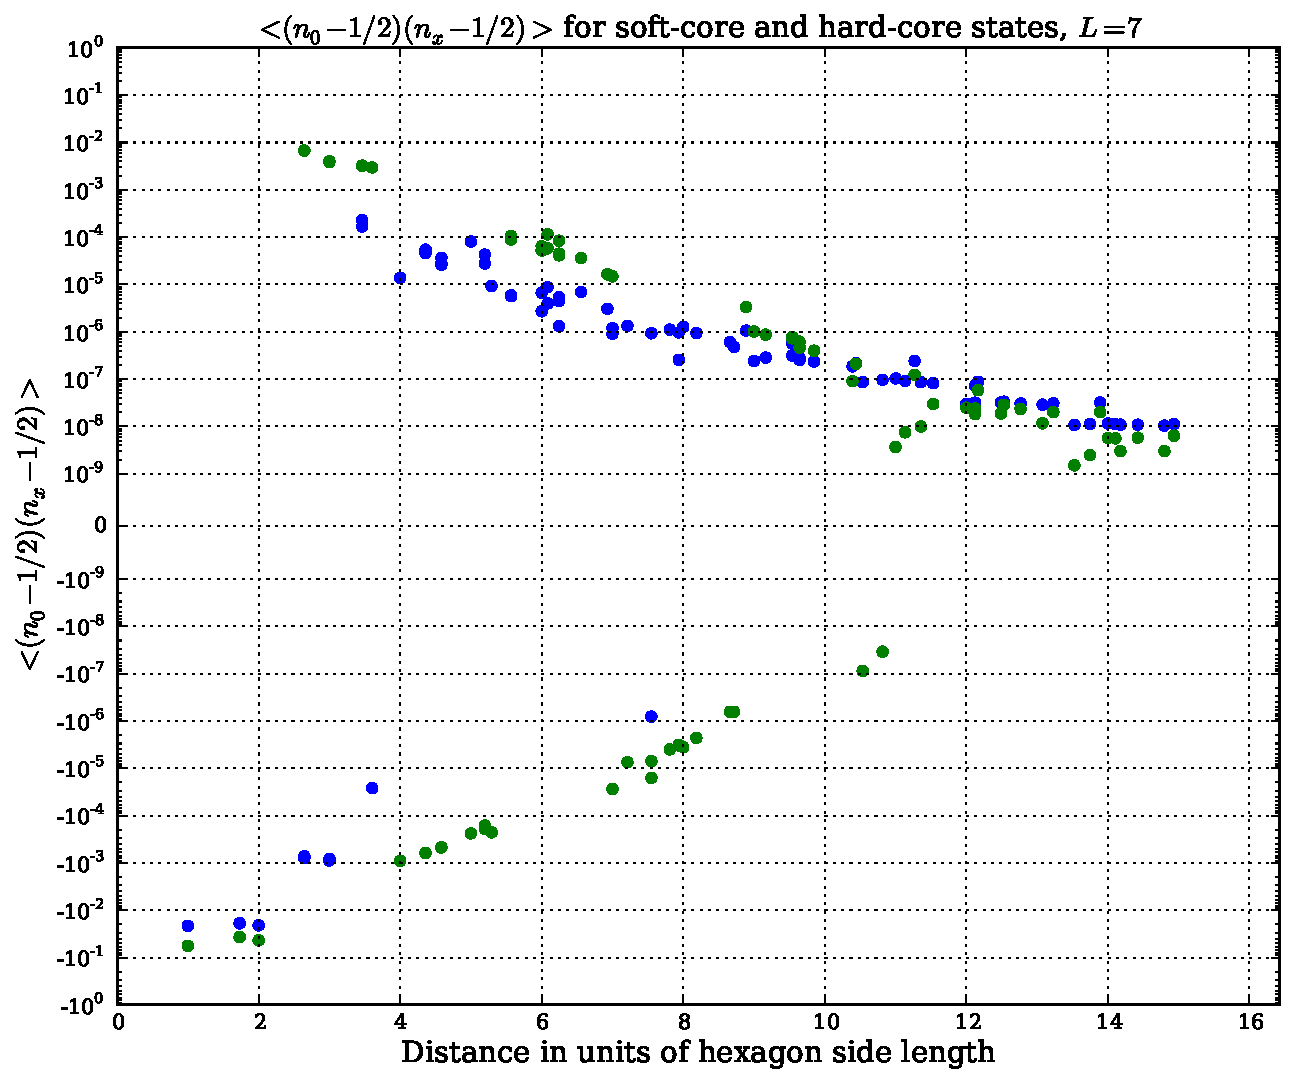
\includegraphics[width=6in]{{summary/log_nn_corr_comparison.pdf}}
\end{center}
\caption{The connected density correlation function $<(n_x - \frac{1}{2})(n_0 - \frac{1}{2})>$ shown on a log-scale for the hard-core (blue) and soft-core (green) boson states. The soft-core state shows some oscillation between positive and negative correlations in density fluctuations, while the hard-core state doesn't as much. Both density fluctuation correlation functions decay very quickly. }
	\label{fig:signed-nn-scatter}
\end{figure}

\begin{figure}[hbctp]
\begin{center}
\includegraphics[width=\textwidth]{{summary/sc-entanglement_spectrum_L8.png}}
\end{center}
\caption{Full entanglement spectrum for the soft-core boson state on the $L=8$ zig-zag edge cylinder. Scale set by making the density matrix have trace 1, i.e. $\sum_i \exp(-E_i) = 1$. The color represents boson number, which can be 0 or 1 for each edge site for this cut. The lone charge 0 state is the lowest energy state.}
\label{fig:sc-entanglement-spectrum}
\end{figure}

\begin{figure}[hbctp]
\begin{center}
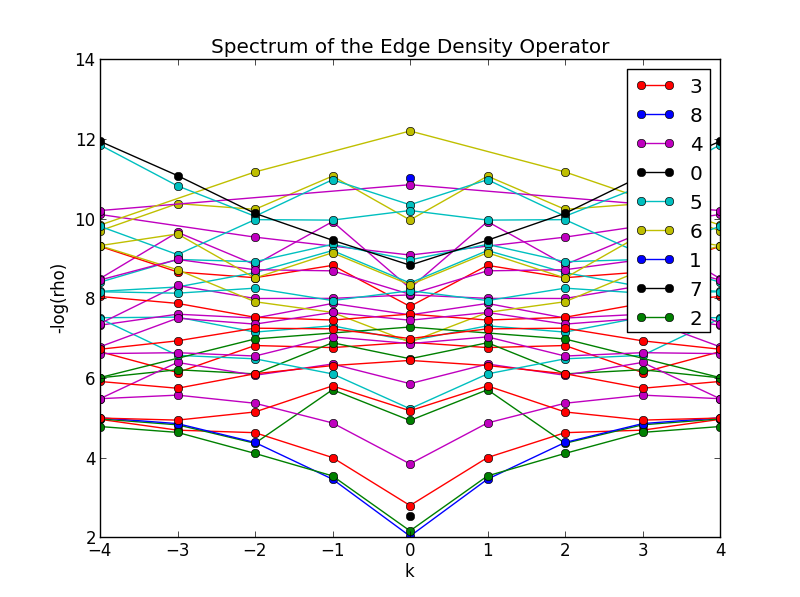
\includegraphics[width=\textwidth]{{summary/hc-entanglement_spectrum_L8.png}}
\end{center}
\caption{Full entanglement spectrum for the hard-core boson state on the $L=8$ zig-zag edge cylinder. The charge 1 state with 0 momentum is the lowest energy state. It looks similar to the soft-core boson entanglement spectrum with a chemical potential shift, i.e. a shift in the energies proportional to the boson-number.}
\label{fig:hc-entanglement-spectrum}
\end{figure}

\begin{figure}[hbctp]
\begin{center}
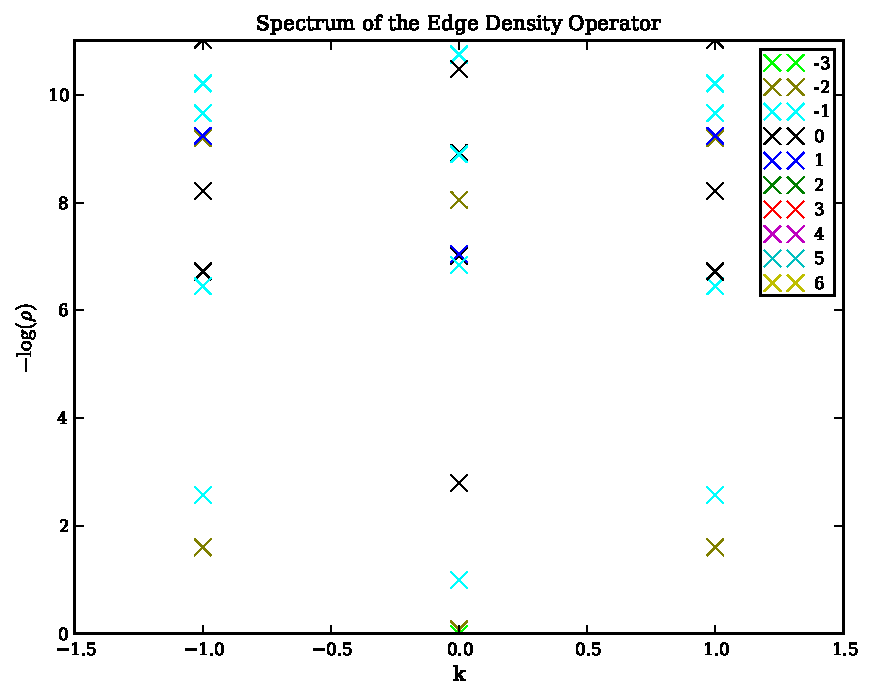
\includegraphics[width=\textwidth]{{armchair_softcoreboson/L3K0N0/edge_spectrum.pdf}}
\end{center}
\caption{Armchair edge entanglement spectrum for the soft-core boson with 6 edge sites. Arbitrary scale.}
\label{fig:armchair-entanglement-spectrumL3}
\end{figure} 

\begin{figure}[hbctp]
\begin{center}
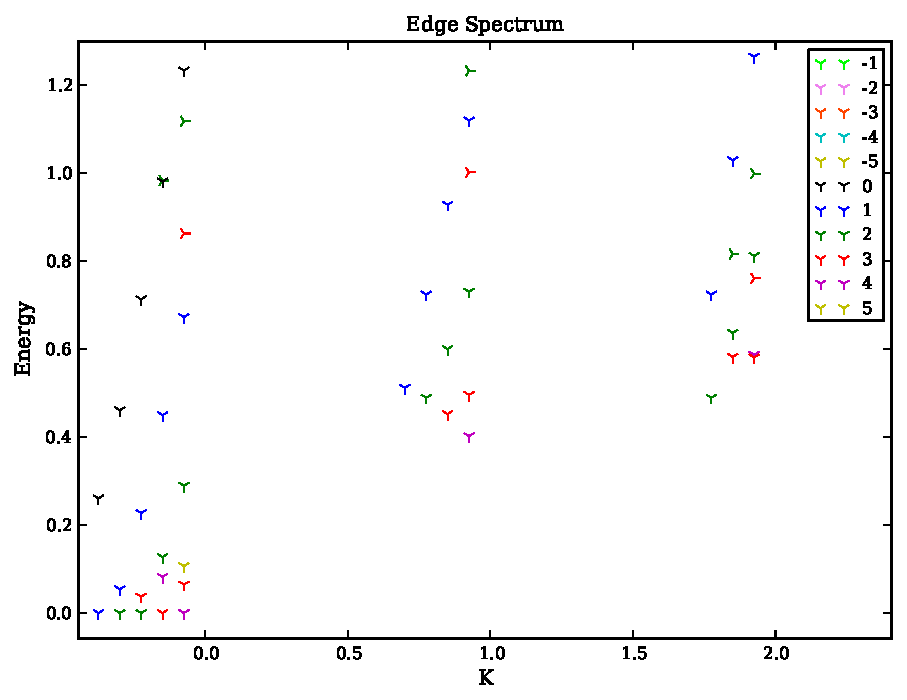
\includegraphics[width=\textwidth]{{rotated_softcoreboson/plots/edge_specL5.pdf}}
\end{center}
\caption{Edge entanglement spectrum for the rotated cut in the soft-core boson with L=1, 2, 3, 4, and 5 edge sites (from left to right.) Not rescaled, but ground state energy shifted to 0. Ground state appears to have charge $L-1$. To create Figure \ref{fig:rotated-entanglement-spectrum}, relabel the charge $N$ state to charge $L-N$, shift the maximum charge states to energy 0, then add a chemical potential shift.}
\label{fig:rotated-entanglement-spectrumL5}
\end{figure}

\newpage
\bibliographystyle{plain}
\bibliography{peps_sources}

%\begin{thebibliography}{9}
%
%\bibitem{lamport94}
%  Leslie Lamport,
%  \emph{\LaTeX: a document preparation system}.
%  Addison Wesley, Massachusetts,
%  2nd edition,
%  1994.
%
%\end{thebibliography}

\end{document}